\section{OSI Model}
\begin{itemize}
    \item What is it?
        \begin{itemize}
            \item OSI Model stands for Open System Intercommincation model.
            \item OSI consists of seven layers, and each layer performs a particular network function.
            \item OSI model was developed by the international organization for standardization (ISO) in 1984.
            \item OSI model divides the whole task into seven smaller and manageable tasks.
            \item Each layer is self contained, so that tasks assigned to each layer can be performed independently.
        \end{itemize}
    
    \item Characteristics of OSI model:
        \begin{figure}[H]
            \centering
            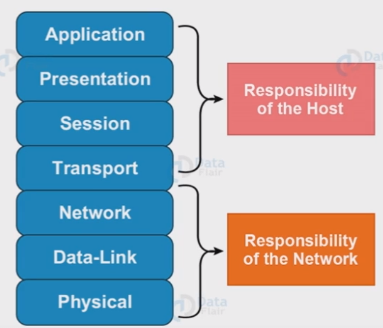
\includegraphics[width=\width\textwidth]{./figs/20230208234631.png}
            %\caption{}
        \end{figure}
        \begin{itemize}
            \item Divided in upper layers and lower layers. The responsability of the host is the tasks assigned to upper layers, and the lower layers are the responsability of the network.
        \end{itemize}
    
    \item Functions of the OSI layers: There are the seven OSI layers. Each layer has different functions.
        \begin{itemize}
            \item Physical layer: transmits raw bit stream over the physical medium.
            \item Data-link layer: Defines the format of data on the network.
            \item Network layer: Decides which physical path the data will take.
            \item Transport layer: Transmits data using transmission protocols including TCP and UDP.
            \item Session layer: Maintains connections and is responsible for controlling ports and sessions.
            \item Presentation layer: Ensures that data is a usable format and is where data encryption takes place.
            \item Application layer: Human-computer interaction layer, where applications can access the network services.
        \end{itemize}
\end{itemize}

%%%%%%%%%%%%%%%%%%%%%%%%%%%%%%%%%%%%%%%%%%%%%%%%%%%%%%
\section{Transmission Control Protocol (TCP/IP)}
\begin{itemize}
    \item What is it?
        \begin{itemize}
            \item TCP is a connection oriented communications protocol that facilitates the exchange of messages between computing devices in a network. It is the most common protocol in networks that use the Internet Protocol (IP); together they are sometimes refered to as TCP/IP.
        \end{itemize}
    
    \item TCP/IP model:
        \begin{itemize}
            \item The TCP/IP model was developed prior to the OSI model.
            \item The TCP/IP model is not exactly similar to the OSI model.
            \item The TCP/IP model consists of five layers: the application layer, transport layer, network layer, data link layer and physical layer.
            \item The first four layers provide physical standards, network interface, internetworking, and transport functions that correspond to the first four layers of the OSI model and these four layers are represented in TCP/IP model by a single layer called the application layer.
            \item TCP/IP is a hierarchical protocol made up of interactive modules, and each of them provides specific functionality.
        \end{itemize}
    
    \item Layers of the TCP/IP model:
        \begin{itemize}
            \item The TCP/IP model is structured with four different layers. These four layers are: 
                \begin{enumerate}
                    \item Network access layer.
                    \item Internet layer.
                    \item Host to host layer.
                    \item Application layer.
                \end{enumerate}
        \end{itemize}
    
    \item Network Access layer:
        \begin{itemize}
            \item This is the bottom layer of the TCP/IP model architecture.
            \item It is a combination of the data link and physical layer of the OSI model.
            \item The physical transmission of data takes place at this layer.
            \item Once the frames are transmitted by a network, encapsylating the IP datagram into these frames is done in this layer.
            \item Also, the mapping of IP address into physical address is done here.
        \end{itemize}
    
    \item Internet layer:
        \begin{itemize}
            \item It is the second layer of the TCP/IP model and this layer is parallel to the network layer of the OSI model in terms of structure.
            \item Sending the data packets to their destination network is the main function of the internet layer.
            \item The logical transmission of data takes place at this level. 
            \item Ther are three different protocols used in this layer.
            \item These include: IP (Internet Protocol), ARP (Address Resolution Protocol), ICMP (Internet Control Message Protocol).
        \end{itemize}
    
    \item Host-to-host layer:
        \begin{itemize}
            \item This layer is parallel to the transport layer of the OSI model.
            \item The error-free delivery of data is the main function of this layer.
            \item There are 2 main protocols present in this layer:
                \begin{itemize}
                    \item TCP: Another integral part, the transmission control protocol is a reliable communication protocol. It manages the flow of data, i.e. the sequence and secmentation of the data.
                    \item UDP: it is a connection-free protocol which makes it cost-effective but less reliable.
                \end{itemize}
        \end{itemize}
    
    \item Application layer:
        \begin{itemize}
            \item The top three layer s of the OSI model: application, presentation and sessions. When combined together, they perform similar functions as the application layer of the TCP/IP model.
            \item node-to-node communcation based on the user-interface occurs here.
            \item Multiple protocols are present in this layer, a few common ones have been mentioned below in brief.
                \begin{itemize}
                    \item HTTP: hypertext transfer protocol is usde to manage the communication between the server and web browsers.
                    \item NTP: network time protocol, can set one standard time source in our computer, which enables sync between the server and the user.
                    \item Telnet: teleommuncation network is used to have access to fils present of in the telnet network and manage them on internet.
                    \item FTP: file transfer protocol, as the name suggests allows easy transferring of files.
                \end{itemize}
        \end{itemize}
\end{itemize}